\chapter{Gráficos do Experimento 1}

\subsubsection{Algoritmo Genético Geracional Clásico}
As Figuras \ref{fig:graphGC1-01}-\ref{fig:graphGC1-10} apresentam a evolução do VPL da melhor solução, da pior solução e a média da população das dez execuções do Algoritmo Genético Geracional Clássico durante o Experimento 1 duarnte a Etapa 1 ($AG^{CC-1}$).

\begin{figure}[H]
\centering
\label{fig:graphGC1-01}
\includegraphics[scale=1]{apxA/aggc/1}
\end{figure}

\begin{figure}[H]
\centering
\includegraphics[scale=1]{apxA/aggc/2}
\end{figure}

\begin{figure}[H]
\centering
\includegraphics[scale=1]{apxA/aggc/3}
\end{figure}

\begin{figure}[H]
\centering

\includegraphics[scale=1]{apxA/aggc/4}
\end{figure}
\begin{figure}[htb]
\centering
\includegraphics[scale=1]{apxA/aggc/5}
\end{figure}


\begin{figure}[H]
\centering

\includegraphics[scale=1]{apxA/aggc/6}
\end{figure}

\begin{figure}[H]
\centering

\includegraphics[scale=1]{apxA/aggc/7}
\end{figure}

\begin{figure}[H]
\centering

\includegraphics[scale=1]{apxA/aggc/8}
\end{figure}

\begin{figure}[H]
\centering

\includegraphics[scale=1]{apxA/aggc/9}
\end{figure}

\begin{figure}[H]
\centering
\label{fig:graphGC1-10}
\includegraphics[scale=1]{apxA/aggc/10}
\end{figure}

\subsubsection{Algoritmo Genético de Regime Permanente}
As Figuras 1-10 apresentam a evolução do VPL da melhor solução, da pior solução e a média da população das dez execuções do Algoritmo Genético de Regime Permanente Clássico durante o Experimento 1 da Etapa 1 ($AG^{RPC-1}$).

\begin{figure}[H]
\centering

\includegraphics[scale=1]{apxA/agrpc/1}
\end{figure}

\begin{figure}[H]
\centering

\includegraphics[scale=1]{apxA/agrpc/2}
\end{figure}

\begin{figure}[H]
\centering

\includegraphics[scale=1]{apxA/agrpc/3}
\end{figure}

\begin{figure}[H]
\centering

\includegraphics[scale=1]{apxA/agrpc/4}
\end{figure}

\begin{figure}[H]
\centering

\includegraphics[scale=1]{apxA/agrpc/5}
\end{figure}

\begin{figure}[H]
\centering

\includegraphics[scale=1]{apxA/agrpc/6}
\end{figure}

\begin{figure}[H]
\centering

\includegraphics[scale=1]{apxA/agrpc/7}
\end{figure}

\begin{figure}[H]
\centering

\includegraphics[scale=1]{apxA/agrpc/8}
\end{figure}

\begin{figure}[H]
\centering

\includegraphics[scale=1]{apxA/agrpc/9}
\end{figure}

\begin{figure}[H]
\centering

\includegraphics[scale=1]{apxA/agrpc/10}
\end{figure}